% Created 2014-01-20 Mon 12:50
\documentclass[12pt]{article}
\usepackage[utf8]{inputenc}
\usepackage[T1]{fontenc}
\usepackage{amsmath,tikz}
\usepackage{amssymb,natbib}
\usepackage{hyperref,setspace}
\onehalfspacing

\usepackage{amsthm}

\newtheorem{lemma}{Lemma}

\title{ Mechanism Design\\\large{Envelope and monotonicity condition in the non-linear pricing model}}
\author{Christoph Schottmüller}
\date{\today}
\usepackage[margin=2.5cm]{geometry}



\begin{document}

\maketitle


\section{Deriving the envelope and monotonicity condition}

We assume that $v$ is twice continuously differentiable. Furthermore, we assume $v_{q\theta }>0$. This assumption is well known under different names (``single crossing condition'', ``Spence-Mirrlees condition'', ``constant sign condition''). This condition will play a major role in the proof of lemma \ref{lem:mon} below.

Now, take an incentive compatible direct revelation mechanism consisting of the two functions $q(\theta )$ and $t(\theta )$. We define $U(\theta )=v(q(\theta ),\theta )-t(\theta )$. As the mechanism is incentive compatible, the following holds for any two types $\theta '$ and $\theta ''$:
\begin{eqnarray*}
  v(q(\theta' ),\theta' )-t(\theta' )&\geq&v(q(\theta'' ),\theta' )-t(\theta'' )\\
v(q(\theta'' ),\theta'' )-t(\theta'' )&\geq&v(q(\theta' ),\theta'' )-t(\theta' ).
\end{eqnarray*}
These two conditions can be rewritten as 
\begin{eqnarray*}
  U(\theta ')&\geq&U(\theta '') -v(q(\theta ''),\theta '')+v(q(\theta ''),\theta ')\\
U(\theta'' )&\geq&U(\theta ') -v(q(\theta '),\theta ')+v(q(\theta '),\theta '').
\end{eqnarray*}
Rearranging these two inequalities gives 
\begin{eqnarray*}
  U(\theta ')-U(\theta '')&\geq& -v(q(\theta ''),\theta '')+v(q(\theta ''),\theta ')\\
U(\theta ')-U(\theta'' )&\leq& v(q(\theta '),\theta ')-v(q(\theta '),\theta '').
\end{eqnarray*}
Assume $\theta '>\theta ''$. Then combining these two inequalities gives
\begin{equation}
  \label{eq:1}
 \frac{ v(q(\theta ''),\theta ')-v(q(\theta ''),\theta '')}{\theta '-\theta ''} \leq \frac{ U(\theta ')-U(\theta '')}{\theta '-\theta ''}\leq \frac{ v(q(\theta '),\theta ')-v(q(\theta '),\theta '')}{\theta '-\theta ''}.
\end{equation}
First we derive the monotonicity constraint: 
\begin{lemma}\label{lem:mon}
  In every incentive compatible mechanism, $\theta '>\theta ''$ implies $q(\theta ')\geq q(\theta '').$ 
\end{lemma}
\textbf{Proof. }(\ref{eq:1}) implies that 
\begin{equation*}
v(q(\theta ''),\theta ')-v(q(\theta ''),\theta '')\leq v(q(\theta '),\theta ')-v(q(\theta '),\theta '')
\end{equation*}
(recall that $\theta '-\theta ''>0$ by assumption). The last inequality can be rewritten as
\begin{equation*}
  \int_{\theta ''}^{\theta '}v_\theta (q(\theta ''),x)\,dx\leq \int_{\theta ''}^{\theta '}v_\theta (q(\theta '),x)\,dx
\end{equation*}
which in turn is equivalent to 
\begin{equation*}
0\leq \int_{q(\theta '')}^{q(\theta ')}\int_{\theta ''}^{\theta '}v_{q\theta} (y,x)\,dx\,dy.
\end{equation*}
By the assumption $v_{q\theta }>0$, the integrand of the previous expression is strictly positive everywhere. But then the previous inequality can (by $\theta ''<\theta '$) hold only if $q(\theta '')\leq q(\theta ')$. (Remember that $\int_a^b\dots=-\int_b^a\dots$.)

Since the types $\theta '$ and $\theta ''$ were arbitrary we get that $q$ has to be monotone, i.e. higher types lead to (weakly) higher decision.\qed

Second, we derive the envelope condition. In (\ref{eq:1}), the right hand side converges to $v_\theta (q(\theta '),\theta ')$ as $\theta ''\rightarrow\theta '$. If $q$ is continuous at $\theta '$, then the left hand side converges to $v_\theta (q(\theta '),\theta ')$ as well. This, of course, implies that the middle term also converges to $v_\theta (q(\theta '),\theta ')$. As the middle term is $U'(\theta )$, we then get $U'(\theta )=v_\theta (q(\theta '),\theta ')$. 
 
As $q$ is monotone (see the lemma above), $q$ is continuous almost everywhere.\footnote{This useful fact follows from the following idea: At every discontinuity $q$ has to ``jump'' over a rational number. If a monotone, say increasing, function had an uncountable number of discontinuities we would therefore have to conclude that there are uncountably many rational numbers (as the function is monotone it has to jump over a different rational at every discontinuity). The rational numbers, however, are countable.  } Consequently, we have shown the following result:
\begin{lemma}[envelope theorem]
  In an incentive compatible mechanism, $U'(\theta )=v_\theta (q(\theta ),\theta )$ for almost all $\theta \in\Theta $ and therefore\footnote{Here we use the fundamental theorem of calculus. Strictly, speaking we have not checked its conditions properly. In particular, we have to verify that $v_\theta (q(\theta ),\theta )$ is bounded and integrable. Without going into details, let me just say that given the assumptions made this can be shown by showing that for $q$ a bounded domain can be used without loss of generality.}
  \begin{equation*}
    U(\theta )=U(0)+\int_0^\theta v_\theta (q(x),x)\,dx.
  \end{equation*}
\end{lemma}

We have now established that incentive compatibility implies both the monotonicity and the envelope condition. Now we want to show the reverse: If a mechanism satisfies both the monotonicity and the envelope condition, then this mechanism is incentive compatible.

Let $t$ and $q$ be such that the envelope contition and monotonicity are satisfied. Take arbitrary types $\theta '$ and $\theta ''$. Because $v_{q\theta }>0$, monotonicity of $q$ implies that
\begin{equation}\label{eq:3}
  \int_{\theta ''}^{\theta '}\int_{q(\theta '')}^{q(x)}v_{q\theta }(y,x)\,dy\,dx\geq 0.
\end{equation}
(The trick is that monotonicity implies $q(x)\geq q(\theta '')$ for all $x\in[\theta '',\theta ']$ if $\theta '>\theta ''$. If $\theta '<\theta ''$, then we can rewrite the expression above as $\int_{\theta '}^{\theta ''}\int^{q(\theta '')}_{q(x)}v_{q\theta }(y,x)\,dy\,dx\geq 0$ and monotonicty implies then that $q(x)\leq q(\theta '')$ for all $x\in[\theta ',\theta '']$.) 

Rewriting (\ref{eq:3}) gives
\begin{equation*}
  \int_{\theta ''}^{\theta '}v_{\theta }(q(x),x)-v_{\theta }(q(\theta ''), x)\,dx\geq 0.
\end{equation*}
By the envelope condition $\int_{\theta ''}^{\theta '}v_{\theta }(q(x),x)\,dx=U(\theta ')-U(\theta '')$, and therefore the previous expression is equivalent to
\begin{equation*}
  U(\theta ')-U(\theta '')-v(q(\theta ''),\theta ')+v(q(\theta ''),\theta '')\geq 0.
\end{equation*}
Rearranging gives 
\begin{equation*}
  U(\theta ')\geq U(\theta '')+v(q(\theta ''),\theta ')-v(q(\theta ''),\theta '')=v(q(\theta ''),\theta ')-t(\theta '').
\end{equation*}
But this simply says that $\theta '$ does not want to misrepresent as $\theta ''$. Since $\theta '$ and $\theta ''$ were arbitrary, the mechanism is incentive compatible which is what we wanted to show.

\section{ ``Single crossing'' and monotonicity: A graphical explanation}

The utility of type $\theta $ when getting quantity $q$ and paying price $t$ is $v(q,\theta )-t$. Think of the consumer's indifference curves in a $q,t$ diagram. Recall that an indifference curve are all the points $(q,t)$ such that $v(q,\theta )-t=\bar{U}$ for some constant $\bar{U}$. The slope of the indifference curve in a point $(q,t)$ is 
\begin{equation*}
  \left.\frac{d\,t}{d\,q}\right|_{U=\bar{U}}=v_q(q,\theta )
\end{equation*}
as can seen from rearranging the equation defining the indifference curve as $t=v(q,\theta )-\bar{U}$.
Intuitively, if we give the consumer one (marginal) unit more, then he is willing to pay $v_q(q,\theta )$ for this additional unit. Hence, we have to charge him $v_q(q,\theta )$ more if we want to keep him indifferent to the starting point.

The single crossing assumption $v_{q\theta }>0$ states that higher types have steeper indifference curves. That is, if the indifference curves of types $\theta '$ and $\theta ''<\theta '$ intersect in one point $(q',t')$ then the curve of $\theta '$ will be steeper and therefore intersect the curve of $\theta ''$ ``from below'' (that is the $\theta '$ curve is below (above) the curve of $\theta ''$ for lower (higher) $q$ than $q'$). Since this is true for any intersection, a given indifference curve of type $\theta '$ can intersect a given indifference curve of type $\theta ''$ only once: Suppose it intersected twice. By what we just said it would have to  intersect both times ``from below''. But as indifference curves are continuous,\footnote{Continuity of the indifference curves follows from the assumed continuity of $v$.} this implies that in between there must be an intersection ``from above''. An intersection from above is, however, impossible by $v_{q\theta }>0$. This contradicts that there is more than one intersection. This is where the name ``single crossing'' comes from.

\begin{figure}[h]
  \centering
  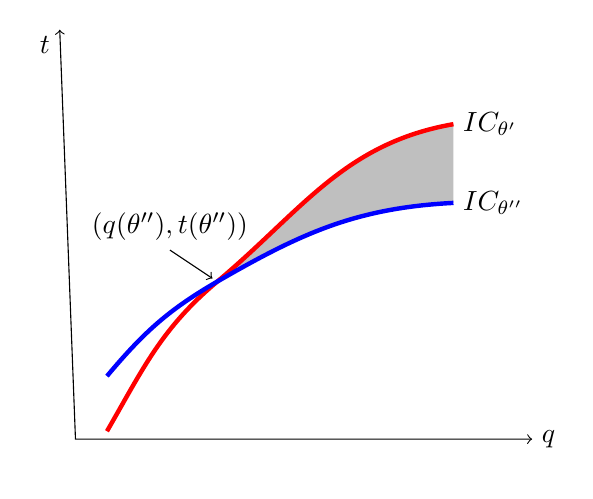
\begin{tikzpicture}[scale=2]
\draw[-] (-0.2,-0.2)--(-0.2,-0.2);
\draw[<->] (3,0)--(0.1,0)--(0,2.6);
\node[right] at  (3,0){$q$};
\node[left] at (0,2.5){$t$};
%\draw[domain=0.3:2.5,thick,blue] plot(\x,{sqrt(\x)});
\path[fill=lightgray, domain=1:2.5]  (1,1) to [out=40,in=190](2.5,2.0) -- (2.5,1.5) to [out = 183,in=30] (1,1);
\draw[ultra thick,red] (0.3,0.05) to [out=60,in=220] (1,1) to [out=40,in=190](2.5,2.0);
\draw[ultra thick,blue](0.3,0.4) to [out=50, in = 210](1,1) to [out=30, in = 183](2.5,1.5);
%\draw[domain=0.3:2.5,thick,red] plot(\x,{2*sqrt(\x)-1});

\node[above] at (.7,1.2){$(q(\theta''),t(\theta''))$};
\draw[->] (.7,1.2)--(.97,1.02);
\node[right] at (2.5,2.0){$IC_{\theta'}$};
\node[right] at (2.5,1.5){$IC_{\theta''}$};
\end{tikzpicture}
  \caption{Single crossing and monotonicity: Indifference curves of $\theta '$ and $\theta ''<\theta '$ through the contract $(q(\theta ''),t(\theta ''))$}
  \label{fig:mon}
\end{figure}

How does this help us to obtain our monotonicity result? In figure \ref{fig:mon} I draw the indifference curves of two types, $\theta ''$ and $\theta '$ with $\theta '>\theta ''$, passing through the contract $(q(\theta ''),t(\theta ''))$ intended for $\theta ''$. As $\theta '>\theta ''$, we have drawn the indifference curve of $\theta '$ -- labeled $IC_{\theta '}$ -- steeper than the indifference curve of $\theta ''$ -- labeled $IC_{\theta ''}$. (This is the role of the single crossing condition $v_{q\theta }>0$ in the figure.)

Where can the contract of type $\theta '$ be if we want the menu to be incentive compatible? In order to be incentive compatible, $\theta '$ has to prefer his own contract $(q(\theta '),t(\theta '))$ to $(q(\theta ''),t(\theta ''))$. Hence, $(q(\theta '),t(\theta '))$ has to be below $IC_{\theta '}$ (recall that right bottom is the direction which the consumer likes better in the $q,t$ diagram: get more, pay less). Incentive compatibility furthermore requires that $\theta ''$ prefers $(q(\theta ''),t(\theta ''))$ over $(q(\theta '),t(\theta '))$. Hence, $(q(\theta '),t(\theta '))$ has to be above $IC_{\theta ''}$. Taking these two requirements together, $(q(\theta '),t(\theta '))$ has to be in the shaded area in figure \ref{fig:mon}. Note that all points in the shaded area have a $q$ above $q(\theta '')$. Hence, $q(\theta ')\geq q(\theta '')$ for any incentive compatible menu -- we obtain the monotonicity condition.

\section{Some remarks on local and global incentive constraints}

Both envelope and monotonicity condition can be regarded as local constraints. That is, under the single crossing assumption, a type does not want to misrepresent as another type if and only if he does not want to misrepresent as a ``closeby'' type. Put differently, if we design a mechanism in which no type is able to benefit from an $\varepsilon $ deviation, then no type can gain froman arbitrary misrepresentation.

To see the local nature of the constraint it is useful to look at the special case in which the function $q$ is continuous and differentiable. In this case, monotonicity and envelope condition can be derived from the first and second order conditions for a local maximum in the optimization problem of the consumer:  The type announcement problem of type $\theta $ can be written as
\begin{equation*}
  \max_{\hat \theta }v(q(\hat{\theta }),\theta )-t(\hat{\theta }).
\end{equation*}
This problem has the first order condition $v_q(q(\hat\theta ),\theta )q_\theta (\hat \theta)-t_\theta (\hat{ \theta })=0$. In an incentive compatible mechanism, the optimal type announcement is the true type and therefore $v_q(q(\theta ),\theta )q_\theta ( \theta)-t_\theta ({ \theta })=0$. To get to the envelope condition, recall that $U(\theta )=v(q(\theta ),\theta )-t(\theta )$ and therefore $U'(\theta )=v_\theta (q(\theta ),\theta )+v_q(q(\theta ),\theta )q_\theta ( \theta)-t_\theta ({ \theta })$. By the first order condition, the difference of the last two terms is 0 in every incnetive compatible mechanism and we get $U'(\theta )=v_\theta (q(\theta ),\theta )$, i.e. the envelope condition.

To get the monotonicity condition, consider the second order condition for a maximum in the consumer's type announcement problem: $v_{qq}(q(\hat\theta ),\theta )q_\theta (\hat \theta)+v_{q}(q(\hat\theta ),\theta )q_{\theta \theta} (\hat \theta)-t_{\theta \theta} (\hat{ \theta })\leq0$ where the left hand side has to be evaluated at the optimum $\hat{\theta }=\theta $ (i.e. assuming incentive compatibility). By the previous paragraph, the first order condition $v_q(q(\theta ),\theta )q_\theta ( \theta)-t_\theta ({ \theta })=0$ holds for every type in an incentive compatible mechanism. Hence, the derivative with respect to $\theta $ of the left hand side has to be zero and we obtain $v_{q\theta }(q(\theta ),\theta )q_\theta (\theta )+v_{qq}(q(\theta ),\theta )q_\theta ( \theta)+v_{q}(q(\theta ),\theta )q_{\theta \theta} ( \theta)-t_{\theta \theta} ({ \theta })=0$. Plugging this back into the second order condition, the second order condition (evaluated at $\hat{\theta }=\theta $) becomes $-v_{q\theta }(q(\theta ),\theta )q_\theta (\theta )\leq 0$. By the assumption $v_{q\theta }>0$, this can only hold if $q_\theta (\theta )\geq 0$, i.e. the monotonicity constraint.

What we have shown is that in an incentive compatible mechanism the envelope and monotonicity constraint hold because they are equivalent to the first and second order condition for a \emph{local} maximum in the type announcement. The striking result that we showed in section 1 is that these two constraints are also sufficient for incnetive compatibility, i.e. the conditions for a local maximum imply a global maximum in our type announcement problem. This property holds only under the single crossing condition $v_{q\theta }>0$. That is, if this condition is violated than complicated non-local incentive constraints can be binding (e.g. type $0.5$ may be indifferent between his menu point and the menu point of type $0.3$ in the optimal mechanism). As this problem is much less tractable, solutions are known only for special cases, see \cite{araujo2010adverse} and \cite{schottmueller2015jet}.

\bibliographystyle{chicago}
\bibliography{/home/christoph/stuff/bibliography/references.bib}

\end{document}

